%!TEX root = Presentation-Thoma.tex

\section{Einfache Lösungsansätze}
\subsection{Einfache Lösungsansätze}
\begin{frame}[t]{Nur Farbinformationen}
    Die Farbe (3 Features, RGB) eines Pixels gibt einen Hinweis darauf, ob es
    sich um ein medizinisches Instrument handelt. Dies wird als Baseline zum
    Vergleich mit anderen Techniken verwendet.

    \begin{table}
    \begin{tabular}{lccc}
    \toprule
    \textbf{Model}        & \textbf{Accuracy} & \textbf{Precision} & \textbf{Recall}   \\ \midrule
    Baseline              & 92.88 \%          & 76.13 \%         & 32.94 \% \\
    \end{tabular}
    \end{table}

    \only<1>{
    Zur Interpretation:
    \begin{itemize}
        \item $\SI{90.5}{\percent}$ sind nicht \enquote{medizinisches Instrument}
        \item $\SI{9.5}{\percent}$ sind medizinisches Instrument
        \item[$\Rightarrow$] $\SI{90.5}{\percent}$ Accuracy sind trivial zu
                             erreichen.
    \end{itemize}
    }
    \only<2>{
    \begin{center}
        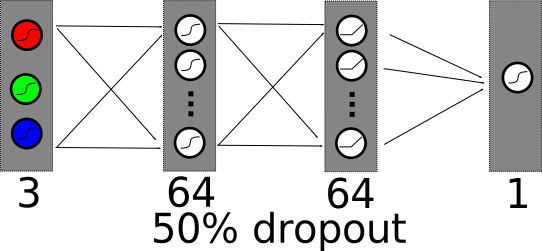
\includegraphics[width=7cm]{../images/model-301-architecture.png}
    \end{center}
    }

\end{frame}

\begin{frame}{Kontext + Morphologische Operationen}
    Ideen:

    \begin{itemize}
        \item Die Farbinformationen der umgebenden Pixel macht das Modell
              robuster.
        \item Morphologische Operationen (öffnen, schließen) machen die lokalen
              Segmentierungsergebnisse global konsistenter.
    \end{itemize}


    \begin{table}
    \begin{tabular}{lccc}
    \toprule
    \textbf{Model}        & \textbf{Accuracy} & \textbf{Precision} & \textbf{Recall}   \\ \midrule
    Baseline              & 92.88 \%          & 76.13 \%         & 32.94 \% \\
                          & {\tiny (+8 \%)}   & {\tiny (+4 \%)}  & {\tiny (+11 \%)}\\
    Local model + opening & 93.42 \%          & 76.98 \%         & 40.65 \% \\
    \end{tabular}
    \end{table}

    Zur Interpretation: +8 \% bedeutet, dass 8 \% des Weges von der Baseline
    zum perfekten Ergebnis zurückgelegt wurden. Also
    $\frac{93.42 - 92.88}{100 - 92.88} \approx 8$.
\end{frame}

\begin{frame}{Ergebnisse Local model + opening}
    \begin{figure}[ht]
        \begin{minipage}[b]{0.45\linewidth}
            \centering
            \includegraphics[width=\textwidth]{../images/model-303/img_02_raw-overlay.png}\\
            \includegraphics[width=\textwidth]{../images/op4-img_01.png}
        \end{minipage}
        \hspace{0.5cm}
        \begin{minipage}[b]{0.45\linewidth}
            \centering
            \includegraphics[width=\textwidth]{../images/model-303/img_06_raw-overlay.png}\\
            \includegraphics[width=\textwidth]{../images/op4-img_05.png}
        \end{minipage}
    \end{figure}
\end{frame}

\begin{frame}{Ergebnisse Local model + opening}
    \begin{figure}[ht]
        \begin{minipage}[b]{0.45\linewidth}
            \centering
            \includegraphics[width=\textwidth]{../images/model-303/img_16_raw-overlay.png}\\
            \includegraphics[width=\textwidth]{../images/op4-img_17.png}
        \end{minipage}
        \hspace{0.5cm}
        \begin{minipage}[b]{0.45\linewidth}
            \centering
            \includegraphics[width=\textwidth]{../images/model-303/img_29_raw-overlay.png}\\
            \includegraphics[width=\textwidth]{../images/op4-img_34.png}
        \end{minipage}
    \end{figure}
\end{frame}
